\documentclass[twocolumn]{article}

\usepackage{graphicx}
\usepackage{fullpage, paralist}


\author{Juli\'{a}n Hern\'{a}ndez, Rodrigo Ipince, Jos\'{e} Mu\~{n}iz}
\title{A Comparison of Algorithms for Self-Tuning Histograms}

\begin{document}

\maketitle


\begin{abstract}
In this paper, we explore the feasibility of implementing self-tuning histograms for OLTP databases. We describe
different algorithm strategies for building and maintaining self-tuning histograms and explore their
performance in an environment of frequent updates over databases with large amounts of data where the current 
model of statistic collection is too costly. 

We conclude by showing that self-tuning histograms provide comparable performance to statistic collection 
with almost no overhead for selectivity estimations over one field. 

\end{abstract}

\section{Introduction}

Traditional database management systems based on the System-R design often include an optimizer. As explained in \cite{astrahan-76}, this optimizer receives a query plan as input and is responsible for evaluating a family of equivalent query plans and choosing a low-cost equivalent for the input plan. In order to estimate the costs of all the feasible plans, the optimizer requires to predict the sizes of intermediate results within the execution of the query before its actual execution. For example, if a join is required between two tables $R$ and $S$, the expected sizes of each relation would dictate the join algorithm to be used. In particular, an optimizer requires knowledge of the distribution of values over different fields. When a query, say, of the form \texttt{SELECT $x_1, x_2, ... , x_n $ FROM T WHERE $P(x_1, x_2, ... , x_n )$}, is entered to the database, the optimizer must approximate the number of tuples in $T$ that satisfy $P(x_1, x_2, ... , x_n )$. We define this expected number of tuples to be the selectivity of $P$, in a way analogous to  \cite{selinger-98}. 

A particular type of selectivity function of interest is the selectivity of predicates of the form $P(x_i) \equiv x_i \in [a,b]$.  These are predicates defined over a single field, and express the fraction of tuples in that field that lie within some range of its domain $[a,b]$. These predicates are common in practice and are also used as building blocks for estimating more complicated multivariable predicates. For example, if $P(x,y)$ is $(x \in [a,b]) \land (y \in [c,d])$ and we assume fields $x$ and $y$ are not correlated, then we can express $P(x,y)$ as $P(x) \times Q(y)$, where $P(n) \equiv   n \in [a,b]$ and $Q(n) \equiv n \in [c,d]$. 

A common approach for estimating these types of selectivities is to use a histogram associated with each field on each relation. Estimating the selectivity from a given query is easy and requires almost no overhead when consulting an already existing histogram. However, the process of building a histogram is usually expensive. Histograms get periodically rebuilt form scratch by an independent component of the database system called the statistics gatherer. This component uses statistical sampling and scans several pages of the table to estimate an approximate distribution of values. This process incurs  significant I/O costs, which makes the operation expensive. Current commercial database systems like Oracle, Microsoft SQL Server, and Sybase, as well as open source alternatives like PostgreSQL and mySQL, all use this approach to single field selectivity estimation, as discussed in \cite{gibbons-97}. When facing large-sized tables with constant updates, statistics analysis can only be performed at low frequencies, which implies the estimates degrade in quality over extended periods of time. Situations of large-sized tables with constant updates may be present in certain kinds of OLTP transactions, which may experience degradation in performance due to the imprecision effects of the histogram. 

Several authors (\cite{aboulnaga-99}, \cite{chen-94}, \cite{christodoulakis-84}) have explored the notion of replacing the independent statistics gatherer with a feedback system by which the results from previous or current queries are fed back to the optimizer for future decision-making. In this paper, we explore some of these works, and propose several modifications for improving the accuracy of these algorithms under our assumptions of large data sets with high frequency updates. We then show that self-tuning histograms represent a viable option for cost estimation under these conditions, and comment on the differences between the different versions of the histogram building algorithms. 

This paper is organized into seven parts. Section \ref{traditional-querying} describes how histograms are used in database systems. Section \ref{prev-work} shows some previous work on using results from queries to improve future cost estimates. Section \ref{our-work} then explains our modifications to the previous algorithms. Finally, Sections \ref{benchmark},  \ref{choice-queries}, and \ref{results} describe our framework for benchmarking these algorithms in a transactional environment. 


\section{Histogram querying and traditional histogram building}\label{traditional-querying}

\subsection{Basic histogram definitions}

In this paper, we use a definition of a histogram similar to  \cite{ionnadis-03} and \cite{ionnadis-95}. Let $V_i$ be the set of possible values of a field $i$, and $f(v), v \in V_i$ be a function that specifies the frequency  (number of tuples where the $i$th field equals $v$) of a given value within a field. Partition the data distribution into disjoint ranges which we call \emph{buckets}. A histogram is then a mapping from each bucket to some frequency, which is computed as some well known function of the frequencies of all values that fall within that bucket. 

Two special type of histograms are commonly used in database management systems, and are described by \cite{gibbons-97}. 

\begin{description}
	\item \emph{Equi-height}: The frequency of any two buckets is equal. In order to represent a non-uniform distribution of values, this type of histogram carefully
			chooses the bucket sizes to preserve the equal frequency discipline. 
	\item \emph{Compact}: In addition to storing the distribution of the complete range of values, an additional histogram stores the most common values and their associated frequencies. 
\end{description}

Postgres uses a \emph{compact} �representation for the most common values of a field, and an \emph{equi-height}� histogram to store the results of the remaining values. 


\subsection{Histograms in the traditional cost model}

In the traditional model, the process of query execution contains three phases:

\begin{description}
	\item[Optimization]  The optimizer uses the histogram generated by the statistics gatherer in order to estimate the costs of different scans and
		then predict the costs of other higher order operations. 
	\item[Execution] Given an optimized query plan, this component is responsible for performing the actual I/O operations and producing the resulting relations. 
	\item[Statistics gatherer] An independent component that runs in parallel and is in charge of updating the histogram. 
\end{description}


	\begin{figure}
	\begin{center}

		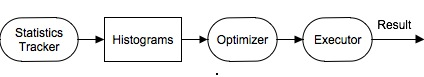
\includegraphics[width=0.9\columnwidth]{traditionalSystem.jpeg}
		\caption{Traditional model for query optimization and execution}	
		\label{fig:traditional-execution}
	\end{center}
	\end{figure}
		
This flow is depicted in Figure \ref{fig:traditional-execution}. We notice that there is no connection between the \emph{traditional-executon} �and \emph{statistics collection} subsystems. 

The optimizer uses the histogram to compute an estimate for the selectivity of a predicate $P(x_i)$ of the form $x_i \in [a,b]$ as follows: 

\begin{itemize}

	\item If range is of type $[a,a]$, then we search in the most common values table. 
		\begin{itemize} 
			\item If it is present, then we can compute its selectivity $\sigma = f(a)$, where $f$ is the frequency function of the most common values histogram.  
			\item If it is not present, then we can estimate its selectivity as 
					$$\frac{\sigma} {\sum_k f(k)} = \frac{1 -  \sum_{k < a}  f(k)} {|b-a| -  \sum_{k < a} 1}  $$
		\end{itemize}
		
		Here, $b$ and $a$ are the end and start range of the bucket where $a$ is located, and $\sum_{k < a} 1$ means the number of most common values less than $a$.
		 In other words, whenever a value is not in the most common values list, we first use the list of most common values to obtain the frequencies of the values less than $a$. 
		 We then estimate the frequency of the remaining unknown values up to $a$ by looking at the \emph{equi-height} histogram and obtaining its frequency. 
		 We divide by $ \sum_k f(k) $ to obtain an absolute number, and not a proportion. 
				
	\item If range is of type $[a,b]$, we follow the same approach as the previous example. In other words, we view the total selectivity as the sum of the frequencies of the values in the range
		 in the most common values list and the frequencies from the \emph{equi-depth}� table of the remaining range. 
	
\end{itemize}

As a simple example, consider a sample \texttt{Students} table. This table contains an \texttt{age} field. Figure \ref{compact-equiheight-histograms} �shows the histograms for the most common values and then for the remaining values.  Now suppose we wish to perform the query \texttt{SELECT * FROM WHERE AGE $\leq 18$}. The shaded areas represent those regions of the histogram which satisfy the predicate.
There are 7 people with a smaller or equal age in the list of most common values.  Therefore, we estimate for the two most common ages a total of 7. For the remaining 16 ages, we use the \emph{equi-height}  histogram and compute an estimated 14 people. Therefore, the selectivity $ \sigma_{h} $  according to the \emph{equi-height}� histogram is 14 and the selectivity  $ \sigma_{MCV} $  according to the most common values histogram is 7. The amount $\alpha$ of people in the range not in the list of common values is $\frac{16}{18} = \frac{8}{9}$ 
 
Therefore, the total number of tuples can be estimated as
$$ \sigma = \alpha�\times \sigma_{h} + \sigma_{MCV} = \frac{8}{9} (14)  + 7 = 19.4  $$ 


	\begin{figure}
	\begin{center}

		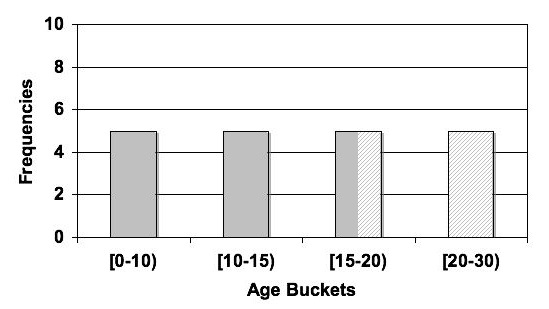
\includegraphics[width=0.8\columnwidth]{chart4.jpg}
		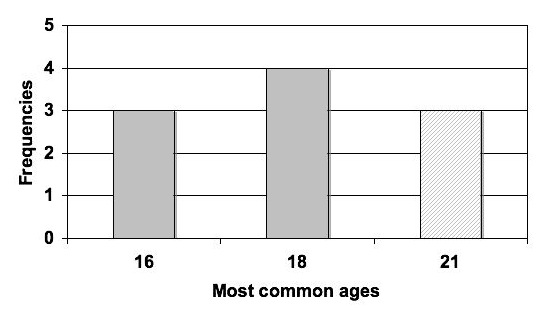
\includegraphics[width=0.8\columnwidth]{chart5.jpg}
		\caption{Compact and equi-height histograms for field \texttt{Students.age}}	
		\label{compact-equiheight-histograms}
	\end{center}
	\end{figure}
	
	
	

It is important to notice that this use of histograms make several key assumptions regarding the data, such as a uniform distribution of values inside of a bucket.  In addition, as described in detail in \cite{christodoulakis-84}, there is an assumption of \emph{query uniformity}, which implies an expectation that queries will refer to all values in a field with equal frequency. 

\subsection{Statistical generation of histograms }�

As described in \cite{gibbons-97}, a statistical approach to building histograms consists of obtaining a set of sample tuples from the relations, performing queries and collecting statistics on this sample set. Although very accurate, 
the process of statistical sampling requires reading a large amount of pages from disk in order to guarantee statistically valid estimations. In Postgres, statistics collections is triggered after some threshold number of insertions, currently 50. 
There are two important trade-offs to consider regarding statistics collections: 

\begin{description}
	\item[Sample size $\leftrightarrow$ performance] The larger the sample size, the more costly it is to generate a histogram. However, this histogram will be more accurate. 
	\item[Sampling frequency $\leftrightarrow$ adaptability] The higher the sampling frequency, the faster the histogram will reflect changes in the distribution of values as they are inserted. 
\end{description}

Unfortunately, the cost of running statistic sampling is prohibitive for large databases. Statistics are gathered during low-load periods. For example, histogram refresh could take place during the end of the day. For the remaining part of the day, these statistics are not updated, resulting in a gradual degradation of cost estimates. 
 
 
\section{Incremental histogram building}\label{prev-work}

	Instead of analyzing the entire table every time the histogram needs to be rebuilt, we consider algorithms that modify the histogram based on recent insertions on updates. 
	
	\subsection{Curve fitting}
	
	A mechanism for self-tuning column selectivity estimates is presented in \cite{chen-94}. This paper presents an algorithm for sequentially approximating attribute value
	distribution by a polynomial that minimizes the sum of the squares of the estimation errors. The described procedure does not use online sampling or offline database
	scans, making it adaptable and showing high accuracy rates.
	
	Although the results from \cite{chen-94} seem promising, they represent a radical shift away from the mechanism described in Section \ref{traditional-querying}. Several pieces of
	software, including subcomponents of the database system and graphical user interfaces for server management rely on the current architecture. For example, in Postgres, 
	applications may interface with the histogram through a regular system table, \texttt{pg\_statistic}, which relies on the currently present architecture. 
	Therefore, a radical shift in the design of any major database system seems unlikely when such a change would achieve performance gains for just some family of data and update frequency conditions. 
	
		

	\subsection{Self-Tuning Histograms}
	
	An extension to the traditional model of optimization depicted in Figure \ref{fig:traditional-execution} is using the result set sizes computed by the query executor to correct for estimation mistakes in the
	histogram. The histogram is then enriched with the free information generated by all operators during the execution phase of the query. In turn, this feedback loop ensures that subsequent queries that 
	contain overlapping predicates have access to better estimates in the future. Figure \ref{self-tuning-execution} shows the modified execution system. The execution component communicates with a histogram
	builder in order to receive information about actual cardinalities between ranges of fields. The histogram can now provide range estimates based on the information received over the query execution lifetime. 
	
	\begin{figure}
	\begin{center}

		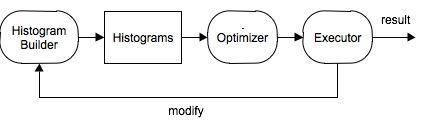
\includegraphics[width=0.9\columnwidth]{stSystem.jpeg}
		\caption{Self-tuning model for query optimization and execution}	
		\label{self-tuning-execution}
	\end{center}
	\end{figure}	
	
		
	The histogram and histogram builder expose the following interface:
	\begin{itemize}
		\item \texttt{receive([a...b], val)}  This function is called by the query executor to inform the histogram builder that there are \texttt{val} values between
		\texttt{a}� and \texttt{b}. 
		\item \texttt{int get([a...b]}  This function asks the histogram to estimate the number of tuples between \texttt{a} and \texttt{b}.
		
	\end{itemize}
	
	In this paper, we disregard the possibility of modifying the query plan while it is being executed, since we expect the number of queries to be so large that it should be possible to see clear performance gains
	by optimizing just future performance. Further, we are interested  not on the performance of a single query but rather the overall throughput of the system. 
	
	Aboulnaga and Chaudhuri describe in \cite{aboulnaga-99} an algorithm for implementing this interface. In doing so, they consider two factors:
	

	\begin{figure}
	\begin{center}

		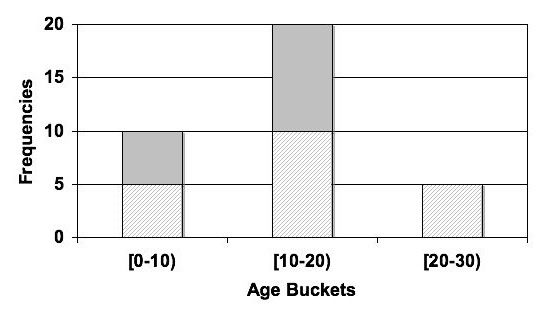
\includegraphics[width=0.8\columnwidth]{chart6.jpg}
		\caption{Histogram modification resulting from a call to \texttt{receive([1,19], 30)}. The shaded region represents a modification to the original histogram}	
		\label{bucket-refinement}
	\end{center}
	\end{figure}
		


	\begin{itemize}
		\item \emph{Bucket refinement}�~ This means updating frequencies for buckets that are found to contain inaccurate information. Figure \ref{bucket-refinement}
		shows a sample histogram refinement for a histogram over an age field in a table of people. Originally, this histogram estimates 15 people of age less than 19. 
		However, the \texttt{receive} call shows that this frequency should actually be 30. In the example, the first two buckets completely cover the range defined in the
		\texttt{receive} call, so they're both updated: the first bucket's frequency is increased by 5 and the second by 10. 
		This reflects the fact that error is distributed in such a way that more error is corrected in buckets with higher frequencies. In other words, \emph{blame} is 
		proportional to frequency. 
		
		\item \emph{Histogram Restructuring}�~�(Merging and splitting buckets) No matter how accurate frequency estimations we obtain for a given range,
			the assumption of uniform distribution of frequencies along a bucket may create large inaccuracies if a bucket contains wide frequency variations. 
			For example, if our table of people were divided in uniform buckets of size 10 between 0 and 100, and the table were to reflect the people working
			for a firm, most buckets would be empty, except for maybe those in the range of 20 to 60. We could obtain a more accurate histogram by using a non-uniform
			bucket distribution in this case.
			
	\end{itemize}
	
		
	\subsubsection{Bucket refinement}�
	The exact algorithm for bucket refinement assigns blame to both range and frequency. Every time a \texttt{receive([a...b], val)} message is passed to the histogram builder, it performs
	the following operations: 
		
	\begin{enumerate}
		\item Calculate the relative error $e$ (percentage of error with respect to estimated result)
		\item For each bucket $b_i$
			\begin{enumerate}
				\item Obtain the fraction $p_i$ of the range \texttt{[a...b]}� represented by $b_i$ 
				\item Set $f(b_i) = f(b_i) ( 1 + \alpha \cdot  e \cdot p_i )  $ 
			\end{enumerate}
	\end{enumerate}
	
	Here $\alpha$ is a damping factor, which is meant to characterize the aggressiveness of our modification; a lower value prevents overfitting. The example presented in Figure \ref{bucket-refinement} 
	shows the special case where $\alpha = 1$. 
	
	\subsubsection{Histogram restructuring}�

	The proposed restructuring method relies on the assumption that splitting high frequency buckets will yield a better histogram. Since the algorithm keeps the number of buckets constant, a separate
	subroutine is responsible for finding buckets to merge, in order to give the opportunity for buckets to split. The histogram restructuring mechanism is triggered after some threshold $T$ number
	of histogram updates. 
	
	\begin{figure}
	\begin{center}

		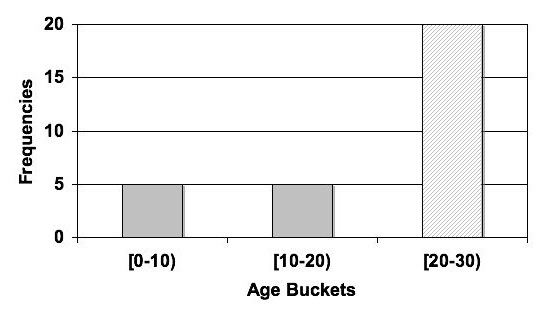
\includegraphics[width=0.8\columnwidth]{chart7.jpg}
		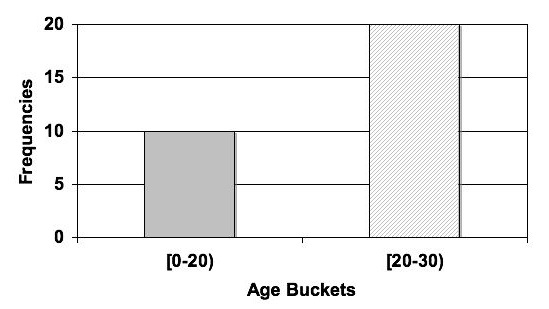
\includegraphics[width=0.8\columnwidth]{chart8.jpg}
		\caption{Histogram merging of two buckets with similar frequency into a single one}	
		\label{bucket-merge}
	\end{center}
	\end{figure}
		


	The policy for merging a bucket is to find pairs of contiguous buckets that have frequency differences smaller than a threshold $M$ between each other. We then merge these two buckets into a single one 
	and repeat this operation until no more buckets can be merged. This algorithm will merge runs of buckets with similar frequencies and will result in the merging of a number
	of buckets, say $k$. 
	
	We decide how we will split each bucket $b_i$ by proportionally assigning splits based on frequency. In other words, the number of buckets after the split for a given bucket
	$b_i$ will be $ \lfloor k \cdot \frac{f(b_i)}{\sum_k f(b_k)} \rfloor $. Figure \ref{bucket-merge} �shows an example of two buckets with similar frequency being merged into a single one. 
	
	
	 	
 
\section{Modifications to proposed algorithms}\label{our-work}

We implemented a modified version of the algorithm proposed in \cite{aboulnaga-99}. In particular, we explore
different strategies with respect to three criteria: 

\begin{description}
	\item[Bucket refinement method] We explore the following possibilities:
		\begin{itemize}
			\item Assignment of blame with respect to frequency alone.
			\item Assignment of blame with respect to range alone.
			\item Hybrid distribution of blame (frequency times range).		 
		\end{itemize}
	\item[Restructuring trigger] We decide to restructure based on two different triggers:
		\begin{itemize}
			\item Number of queries.
			\item Cumulative error (When the amount of error that has been assigned to a 
				given bucket exceeds some threshold).
		\end{itemize}
	\item[Split selection method]�
		\begin{itemize}
			\item Split highest frequency buckets (as in  \cite{aboulnaga-99}).
			\item Split buckets based on their cumulative errors. Buckets store the cumulative error that has been
				blamed on them, and then we split the ones that have accumulated the most error,
				since they have failed to meet estimates more often.
			\item Split buckets based on their usage. More frequently used buckets will be split first. This ensures
				that the buckets the user has been querying the most often are given higher priority and the range
				estimates are stored in more detail.
		\end{itemize}
\end{description}�


\section{Benchmark setup}\label{benchmark}

In order to test the accuracy of the previously discussed algorithms for self-tuning histograms, we built a system as shown in Figure \ref{pwngres-system} on top of Postgres. Postgres was chosen because of three reasons: 

\begin{enumerate}
	\item It is a widely used, open source database system that implements histogram based cost estimation with statistics collection. 
	\item \texttt{EXPLAIN ANALYZE} �provides an easy interface for obtaining query plans for a given query. 
	\item The choice of database is not the main focus of the paper, since the results show the differences between different histogram building algorithms in the presence of large amounts of data and high insertion rates,
		regardless of platform choice. Further, although we do use the statistics analyzer from Postgres, we assume the most popular database systems have highly accurate statistics gatherers. 
\end{enumerate}

\begin{figure}
\begin{center}

	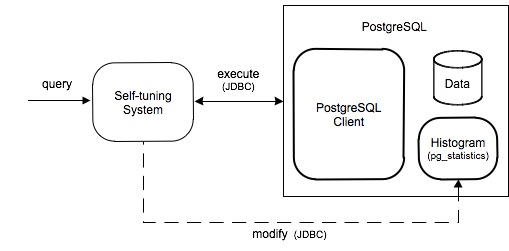
\includegraphics[width=0.8\columnwidth]{systemDiagram.JPEG}
	\caption{High level overview of the benchmarking system}	
	\label{pwngres-system}
\end{center}
\end{figure}

This system represents an intermediate layer between the end user and Postgres, which intercepts the results from the database to the user and uses the cardinality to build a histogram. The different histograms can then be compared by their accuracy.

Our system is responsible for receiving user queries. The information is then fetched back to Postgres, which responds to the middle system with the query plan to be executed. The benchmark tool then simulates the query plan, by reducing it into a family of nested loop joins and sequential scans with a set of conditions. For each query, a collection of \texttt{receive} calls is sent to the histogram builder. For each scan, the executor makes one \texttt{receive} call. In the case of a join, for each element in the outer loop, the executor can make a \texttt{receive} call as it matches the join field in the outer table with the tuples in the inner table. For example, if Tables \ref{emptable} and \ref{depttable} are joined by a natural join, where \textbf{Employees} is the outer table, then we get the following three distinct \texttt{receive} calls: 

\begin{verbatim}
	 receive(``Dept.Country'', [3...3], 2)
	 receive(``Dept.Country'', [2...2], 0) 
	 receive(``Dept.Country'', [1...1], 1) 
\end{verbatim}
	
	\begin{table}
	\begin{center}
	\begin{tabular}[t]{|c|c|}
		\hline
		\textbf{EmpID} & \textbf{Country} \\
		\hline	
			1 		& 3			 \\
			2 		& 2			 \\
			3 		& 2			 \\
			4 		& 1			 \\
		\hline
	\end{tabular}
	\end{center}
	\caption{Table for 	\textbf{Employees}}
	\label{emptable}
	\end{table}
	
	\begin{table}
	\begin{center}
	\begin{tabular}[t]{|c|c|}
		\hline
		\textbf{DeptID} & \textbf{Country} \\
		\hline	
			1 		& 3		          \\
			2 		& 3			 \\
			3 		& 1			 \\
		\hline
	\end{tabular}
	\end{center}
	\caption{Table for \textbf{Departments}}
	\label{depttable}
	\end{table}


The system assumes independence between selectivities of multiple conditions, either over a single table or over several tables. In other words, if a query of the form \texttt{SELECT ... WHERE $p_1$ and $p_2$}, we assume that $\sigma_{p_1} \times \sigma_{p_2} = \sigma_{p_1 \land p_2}$.  For this reason, the join algorithms can be modified to send \texttt{receive} messages even when facing multiple conditions, especially when one is a join condition and the other is a filter on the data. Any computation of \texttt{receive} messages occurs with almost no overhead, since the data it uses needs to be derived by the query executor anyways. 

The middle layer strategy for the benchmark system was chosen over direct modification of Postgres because of the following reasons: 

\begin{itemize}
	\item From the viewpoint of the histogram builder, the messages received from the executor of different join strategies will be equivalent. Therefore, when calculating the change of error rates
	as a result of these messages, only one type of join needs to be considered. 
	\item  When computing error rates of row selectivity estimates, we need not consider the overhead between inter-application connections. 
	\item Since Postgres uses an \emph{equi-depth} histogram, storing the results in Postgres would imply modifying the system catalog slightly to store the additional frequency table. 
	We should note, however, that because of the heuristic with which we merge and split buckets, the algorithm converges to an \emph{equi-depth} histogram. Because of the fast speed of convergence
	demonstrated in Section \ref{results}, this means that storing the histogram without associated frequencies will not significantly impact the accuracy of its estimations. For this reason, a compression scheme
	may be possible for tables with non-changing distributions in order to eliminate the need of a frequency table. This option was not presently explored.

\end{itemize}

Finally, it should be noted that we choose to measure our results in terms of row estimate errors, instead of query execution times. This decision was taken for several reasons:

\begin{itemize}	
	\item The \texttt{pg\_statistic} table in Postgres, which is responsible for holding
		the histogram information, is not modifiable through an external interface. Although
		this histogram is stored in a regular table, the schema uses \texttt{anyarray} as the type
		for the histrogram buckets column, which makes it impossible to change except from the 
		Postgres C libraries. 
		
	\item Although small differences in estimation between the self-tuning system and the conventional
		Postgres system may be irrelevant, order of magnitude differences are certain to be significant
		when scanning over data that contains several types of indices and therefore multiple scanning
		strategies for the optimizer to pick. Similarly, these differences will dictate the strategies for joining
		and aggregating data. 
		
	\item Estimate errors, in contrast with query execution times, represent a database independent metric of
		performance. 
	
\end{itemize}

\section{Choice of Queries and Insertions}\label{choice-queries}

We use a framework of insertions in the spirit of the TPC-W benchmark (see \cite{garcia-03}), modeling an online transaction business. However, unlike TPC-W, we assume the number of products changes very frequently. This situation could arise in an online system similar to online auction sites like eBay. Our benchmark includes the following tables: 

% Quote TPC-W spec here 

\begin{enumerate}
	\item \texttt{Auctions(auc\_id, owner\_id, category\_id, time\_start, time\_end, winning\_bid)}   
	\item \texttt{Users(uid, name)}  
	\item \texttt{Category({category\_id}, description)}  
\end{enumerate} 

The \texttt{Auctions} �relation stores all the items on sale posted by any user of the system. It contains information about its owner, start and end times for the auction, as well as the current winning bid. The \texttt{Users}  relation contains the list of all users of the systems, acting as buyers, sellers or perhaps both. Finally, the \texttt{Category}� relation stores the types of products being auctioned. A possible category could be a particular brand of laptop, which could appear several times in the \texttt{Auctions} if it is being sold by several users at the same time. 

We use similar transactions as defined in the TPC-W specification, disregarding those that involve lookups on primary keys. The lookups on primary keys can readily be estimated to have a result set size of at most one, and therefore would not yield any interesting results. For this reason, we only consider the following four transactions: 



\begin{asparaenum}[\textbf{Transaction} 1 \textbf{:}] 
	\item \emph{Insert auction}.  Inserts a new auction. The product and customer of this inserted auction is uniformly drawn from the table of customers and the table of products. The start date is the insertion time, 
								 		while the end date is a normally distributed random variable with mean of one day after the insertion time and standard deviation of a third of a day.  This transaction
										simulates a user creating a new online auction, and is therefore classified as a frequent write transaction.
	\item \emph{Expired auctions query}.  Selects the auctions that have expired at the point the transaction runs. This transaction simulates an ETL process that moves old information from this table into a data warehouse. 
	\item \emph{Current auctions query}. Selects the auctions that are set to expire within one day of the time that transaction runs. This transaction simulates a likely query executed by a user who wishes to know information
								about current auctions that are close to expiring. 
	\item \emph{Product query}. Counts the number of auctions that correspond to a product that is drawn at random from the list of all products. This transaction simulates a query executed for a particular product in the system. 

\end{asparaenum}

We simulate the execution of this database over a day. The tables are pre-populated with 10,000 products, 5,000 users, and 100,000 records in the auctions table. The transactions are executed as follows:

\begin{itemize}
	\item Every second, \emph{Insert auction}� is executed.
	\item Every thirty seconds, we additionally execute \emph{Product query}.
	\item Every minute, all remaining transactions are executed.
\end{itemize}

We disable the statistics analyzer from Postgres during the execution of the benchmark, but run a full \texttt{VACUUM} and \texttt{ANALYZE} just prior to it. This condition simulates a daily statistics collection process under conditions where
the statistics collection process is too costly to run frequently. In order to benchmark the results, we make the following comparisons: 

\begin{itemize}
	\item We execute queries and insertions on the benchmarking system described in Section \ref{benchmark}. The benchmarking system is run once for each of the different algorithm types to be tested. 	
		As described in Section \ref{benchmark}, this subsystem will automatically generate the \texttt{receive} messages to update the histograms. We measure the error rate of a given query as the average
		error on selectivity estimation defined over a single field. 
		
	\item  We perform the same queries and insertions (in the same order) directly into Postgres. Using \texttt{EXPLAIN ANALYZE}, we define the average difference between actual and real row count over
		scans. These two definitions of error are equivalent since the query plans on both systems take the same form, and therefore would send the same \texttt{receive} and \texttt{get} messages to a histogram
		builder.  

\end{itemize}
  
We ran the benchmark using a different version of bucket refinement, restructuring trigger, and split selection. We assume that the performance of each of the modifications is independent, so it is not necessary to run all possible combinations of refinements. 



% We 
% for (time t in now to now + 1 day)
%       run T1    
%       run T2 if t marks the start of a minute
%	 run T3 and T4 if t marks the half of a minute
%
%
%
%
%

\section{Results}\label{results}

For brevity, we present the most significant results, related to the split selection mechanisms. The results from the bucket refinement confirm the hypothesis from \cite{aboulnaga-99} that there's close to a twofold accuracy gain by using both frequency and range distributed blame instead of range or frequency alone. The restructuring trigger modification yielded no significant performance differences. We now present the results from benchmarking the self-tuning algorithm with three different split selection algorithms against the static histogram built by the statistics gatherer in Postgres. These split selection algorithms were defined in Section \ref{our-work}. 

The figures labeled \emph{Number of rows} represent the actual average cardinality of the tables versus the time of the day when the query was executed. These compare Postgres's own row count estimation against the three benchmarked algorithms for self-tuning histograms and the real row count. The \emph{Absolute error} graphs show the difference between the estimated and actual row count as a function of the time of the day at which they were executed. The same lines as in the row count are present.  


\subsection{Expired auctions query}
\begin{figure}
\begin{center}

	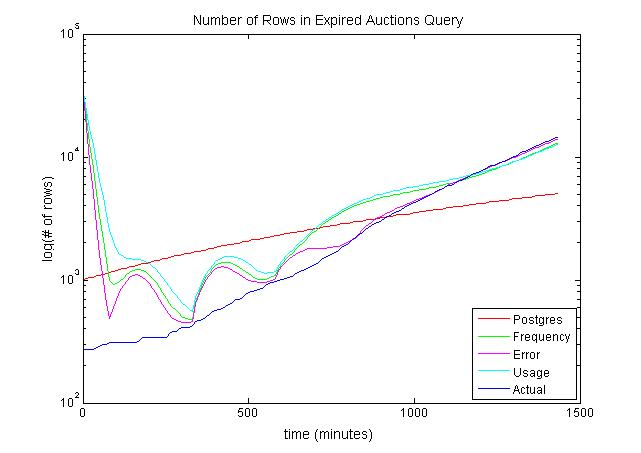
\includegraphics[width=\columnwidth]{query2rows.jpg}
	\caption{Number of rows for \emph{Expired auctions} query}	
	\label{results_query2}
\end{center}
\end{figure}



Figure \ref{results_query2} shows the row count for the expired auctions. The cardinality of the result set of this query should be increasing with time, since existing auctions will expire as time goes on. We notice that the self-tuning histogram estimates follow the actual values closely. The estimates are as close as 50 tuples apart in less than 400 queries. However, the estimates oscillate before they finally stabilize. We attribute the oscillation to under-damping in the histogram bucket frequency refinement phase. 

The initial estimates for all three self-tuning histograms are inaccurate. This happens because the histograms have not yet received any feedback from the queries, so the histogram is initialized with all buckets of the same size and equal frequencies.

%Indeed, at time 0 in the graph, there are 100,000 tuples in the \texttt{Auctions} table, all of which expire roughly 1 day after they were created. Thus, the initial estimate is of roughly 30,000 tuples 
%(WTF? It should be like 15,000).


\begin{figure}
\begin{center}

	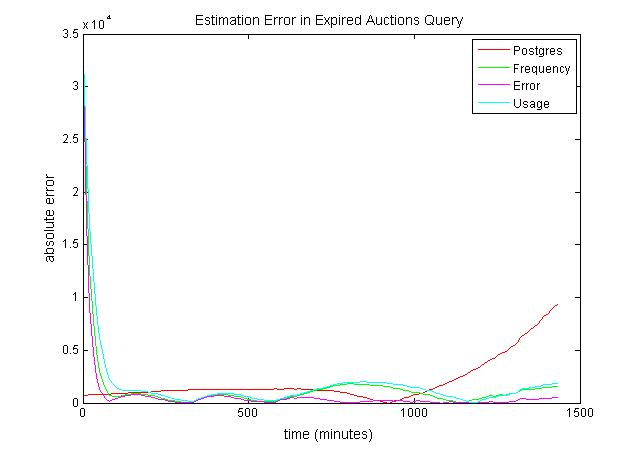
\includegraphics[width=\columnwidth]{query2error.jpg}
	\caption{Absolute error for \emph{Expired auctions} query}	
	\label{error_query2}
\end{center}
\end{figure}





Figure \ref{error_query2} plots the absolute estimation error obtained for the same query. Notice that the error of Postgres is relatively low for the first two thirds of the day, at which point it starts increasing rapidly. This behavior is expected since Postgres has information about the tuples that were already in the \texttt{Auctions} table at $t = 0$. The tuples that are added after $t = 0$ do not affect the query until they start expiring, and this only starts happening towards the end of the day because of the way we constructed the expiration dates for the auctions (normally distributed at 1 day with standard deviation of $\frac{1}{3}$ of a day).

Notice that this query constantly consults a very large number of buckets at a given time. For this reason, the \emph{usage split} algorithm may be outperformed by the other self-tuning algorithm variations, since most buckets are being queried and thus are equally likely to split. We conjecture that the \emph{error split}� algorithm outperforms the \emph{frequency split}  algorithm whenever there are enough queries to provide significant feedback to the histogram about the error distributions in the histogram. This is because the \emph{frequency split} heuristic is only based on the idea that higher frequencies are related to higher error, whereas the \emph{error split}  heuristic is based on actual error data.  It should be noted, however, that all three algorithms converge quickly to the desired result. 


\subsection{Current auctions query}

\begin{figure}
\begin{center}

	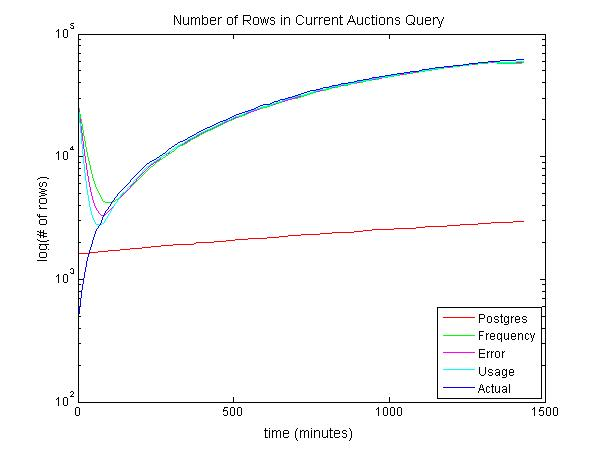
\includegraphics[width=\columnwidth]{query3rows.jpg}
	\caption{Number of rows for \emph{Current auctions} query}
	\label{results_query3}
\end{center}
\end{figure}

\begin{figure}
\begin{center}

	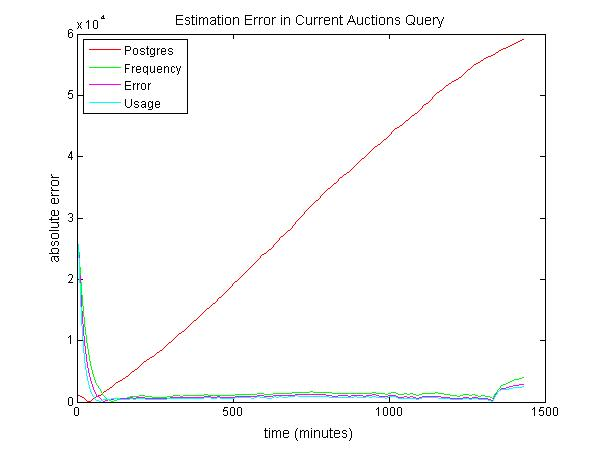
\includegraphics[width=\columnwidth]{query3error.jpg}
	\caption{Absolute error for \emph{Current auctions} query}	
	\label{error_query3}
\end{center}
\end{figure}




Figures \ref{results_query3} and \ref{error_query3} show the graphs outlining the results of the \emph{Current auctions} query. We can notice a similar pattern of quick convergence to a low error and a gradual decay of Postgres's estimation accuracy. In this case, however, the insertion of new elements has an immediate adverse effect on the accuracy of Postgres's selectivity estimation. This is a result of the newly introduced auctions, many of which satisfy the predicate for this query. 

Notice that this time the queries focus on a much smaller range, and then do not go back to older ranges again. For this reason, the \emph{usage split} algorithm can probably exploit this fact to expand the buckets that are being currently used in order to provide better estimates. The \emph{frequency split} �algorithm still outperforms the \emph{error split}  algorithm in this situation. 

\subsection{Product query}


\begin{figure}
\begin{center}

	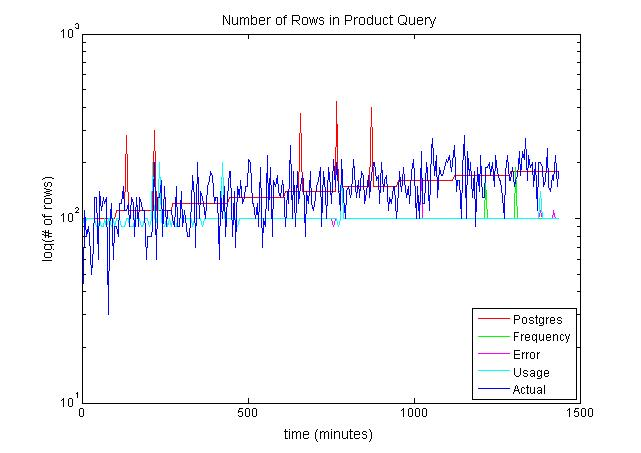
\includegraphics[width=\columnwidth]{query4rows.jpg}
	\caption{Number of rows for \emph{Product} query }	
	\label{results_query4}
\end{center}
\end{figure}

\begin{figure}
\begin{center}

	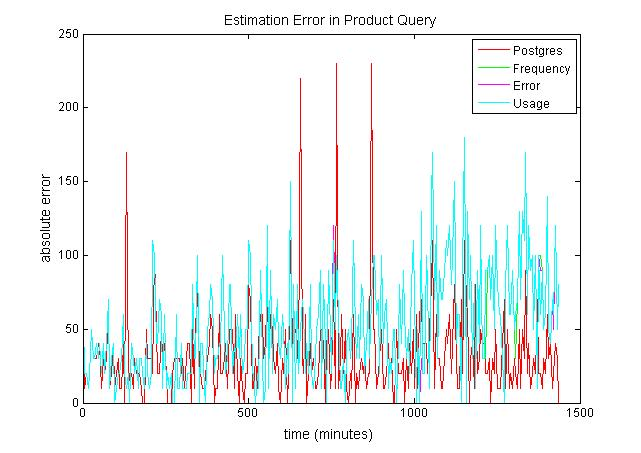
\includegraphics[width=\columnwidth]{query4error.jpg}
	\caption{Absolute error for \emph{Product} query}
	\label{error_query4}
\end{center}
\end{figure}



The last pair of graphs, shown in Figures \ref{results_query4} and \ref{error_query4}, depict the performance on the \emph{Product query}. The three self-tuning histograms estimate the same number of tuples (around 10) consistently. In this case, refinement does not work properly because the errors are so small (around 5) and the per-bucket frequencies are so large (around 1000 or 500, depending on whether we use 10 or 20 buckets, respectively), that bucket refinement does not have a significant impact during estimation. Moreover, since the histogram computed the previous day contains all the products, and the distribution of products over the auctions table does not change over time, the histogram collected by Postgres is expected to continue being a good estimate. 



\section{Conclusion}

In this paper, we discussed a very efficient family of algorithms for computing cardinality estimates over a single field. We showed that self-tuning histograms may be useful for high frequency update data stores that need to hold large amounts of data and thus make a regular statistics collection system prohibitively expensive. These high frequency updates must also change the distribution of values over time at a speed much larger than the histogram update frequency.  Since building histograms based on query feedback modifies a constant-sized histogram with a relatively small amount of buckets, this means that we may update the histogram very frequently without worrying about performance hits. 

We also concluded that a histogram building discipline that distributes blame based on both frequency and range is vastly superior to one that only considers range or frequency when deciding how to update frequencies. In a similar manner, there appears to be a slight accuracy improvement by splitting buckets that are more used whenever the number of used buckets is small with respect to the histogram. Further, there is a slight improvement to splitting buckets when the bucket frequency is high by splitting it when the bucket has been corrected very often. This may be a result of using actual feedback data as a means to determine which buckets to split, instead of the simple assumption that higher frequencies may correspond to higher error rates in the histogram. 

It should be noted, however, that self-tuning based systems that operate on unchanging range distributions or in read-mostly environments may be outperformed by a regular statistics collection mechanism, since the amount of statistics that require to be collected would be very small with respect to the number of queries.	Furthermeore, in most of this report, we have disregarded the effect of errors during estimations of join selectivities. Although self-tuning histograms could provide a good framework for developing multi-dimensional histograms, this option was not explored here. Further, join selectivity errors could well prove to be the driving bottleneck for performance optimization in real systems. 
A final remark is that the use of self-tuning histogram does not ease the impossibility of using histograms in certain class of one field predicates, such as those using \texttt{LIKE}. These queries still require to use alternative estimation mechanisms. 


%Mechanism is only useful when you insert a lot of data that varies the distribution of field values over time. 
%No significant impact between . 

\bibliographystyle{acm}
\bibliography{Biblio}


\end{document}

%why this vs cq model. optimal for oltp txns with large loads, join selectivity still fails. 